%! Author = Mateusz
%! Date = 08/12/2025

\subsection{Projekt strony głównej}
\label{subsec:projekt-strony-glownej}

Na potrzeby strony głównej aplikacji zaprojektowano dwa warianty widoku:
prosty (rys. \ref{img:simple-home-page}) oraz zaawansowany
(rys. \ref{img:advance-home-page}), tak aby możliwe było dopasowanie
sposobu wyszukiwania do preferencji użytkownika.

\begin{figure}[H]
    \centering
    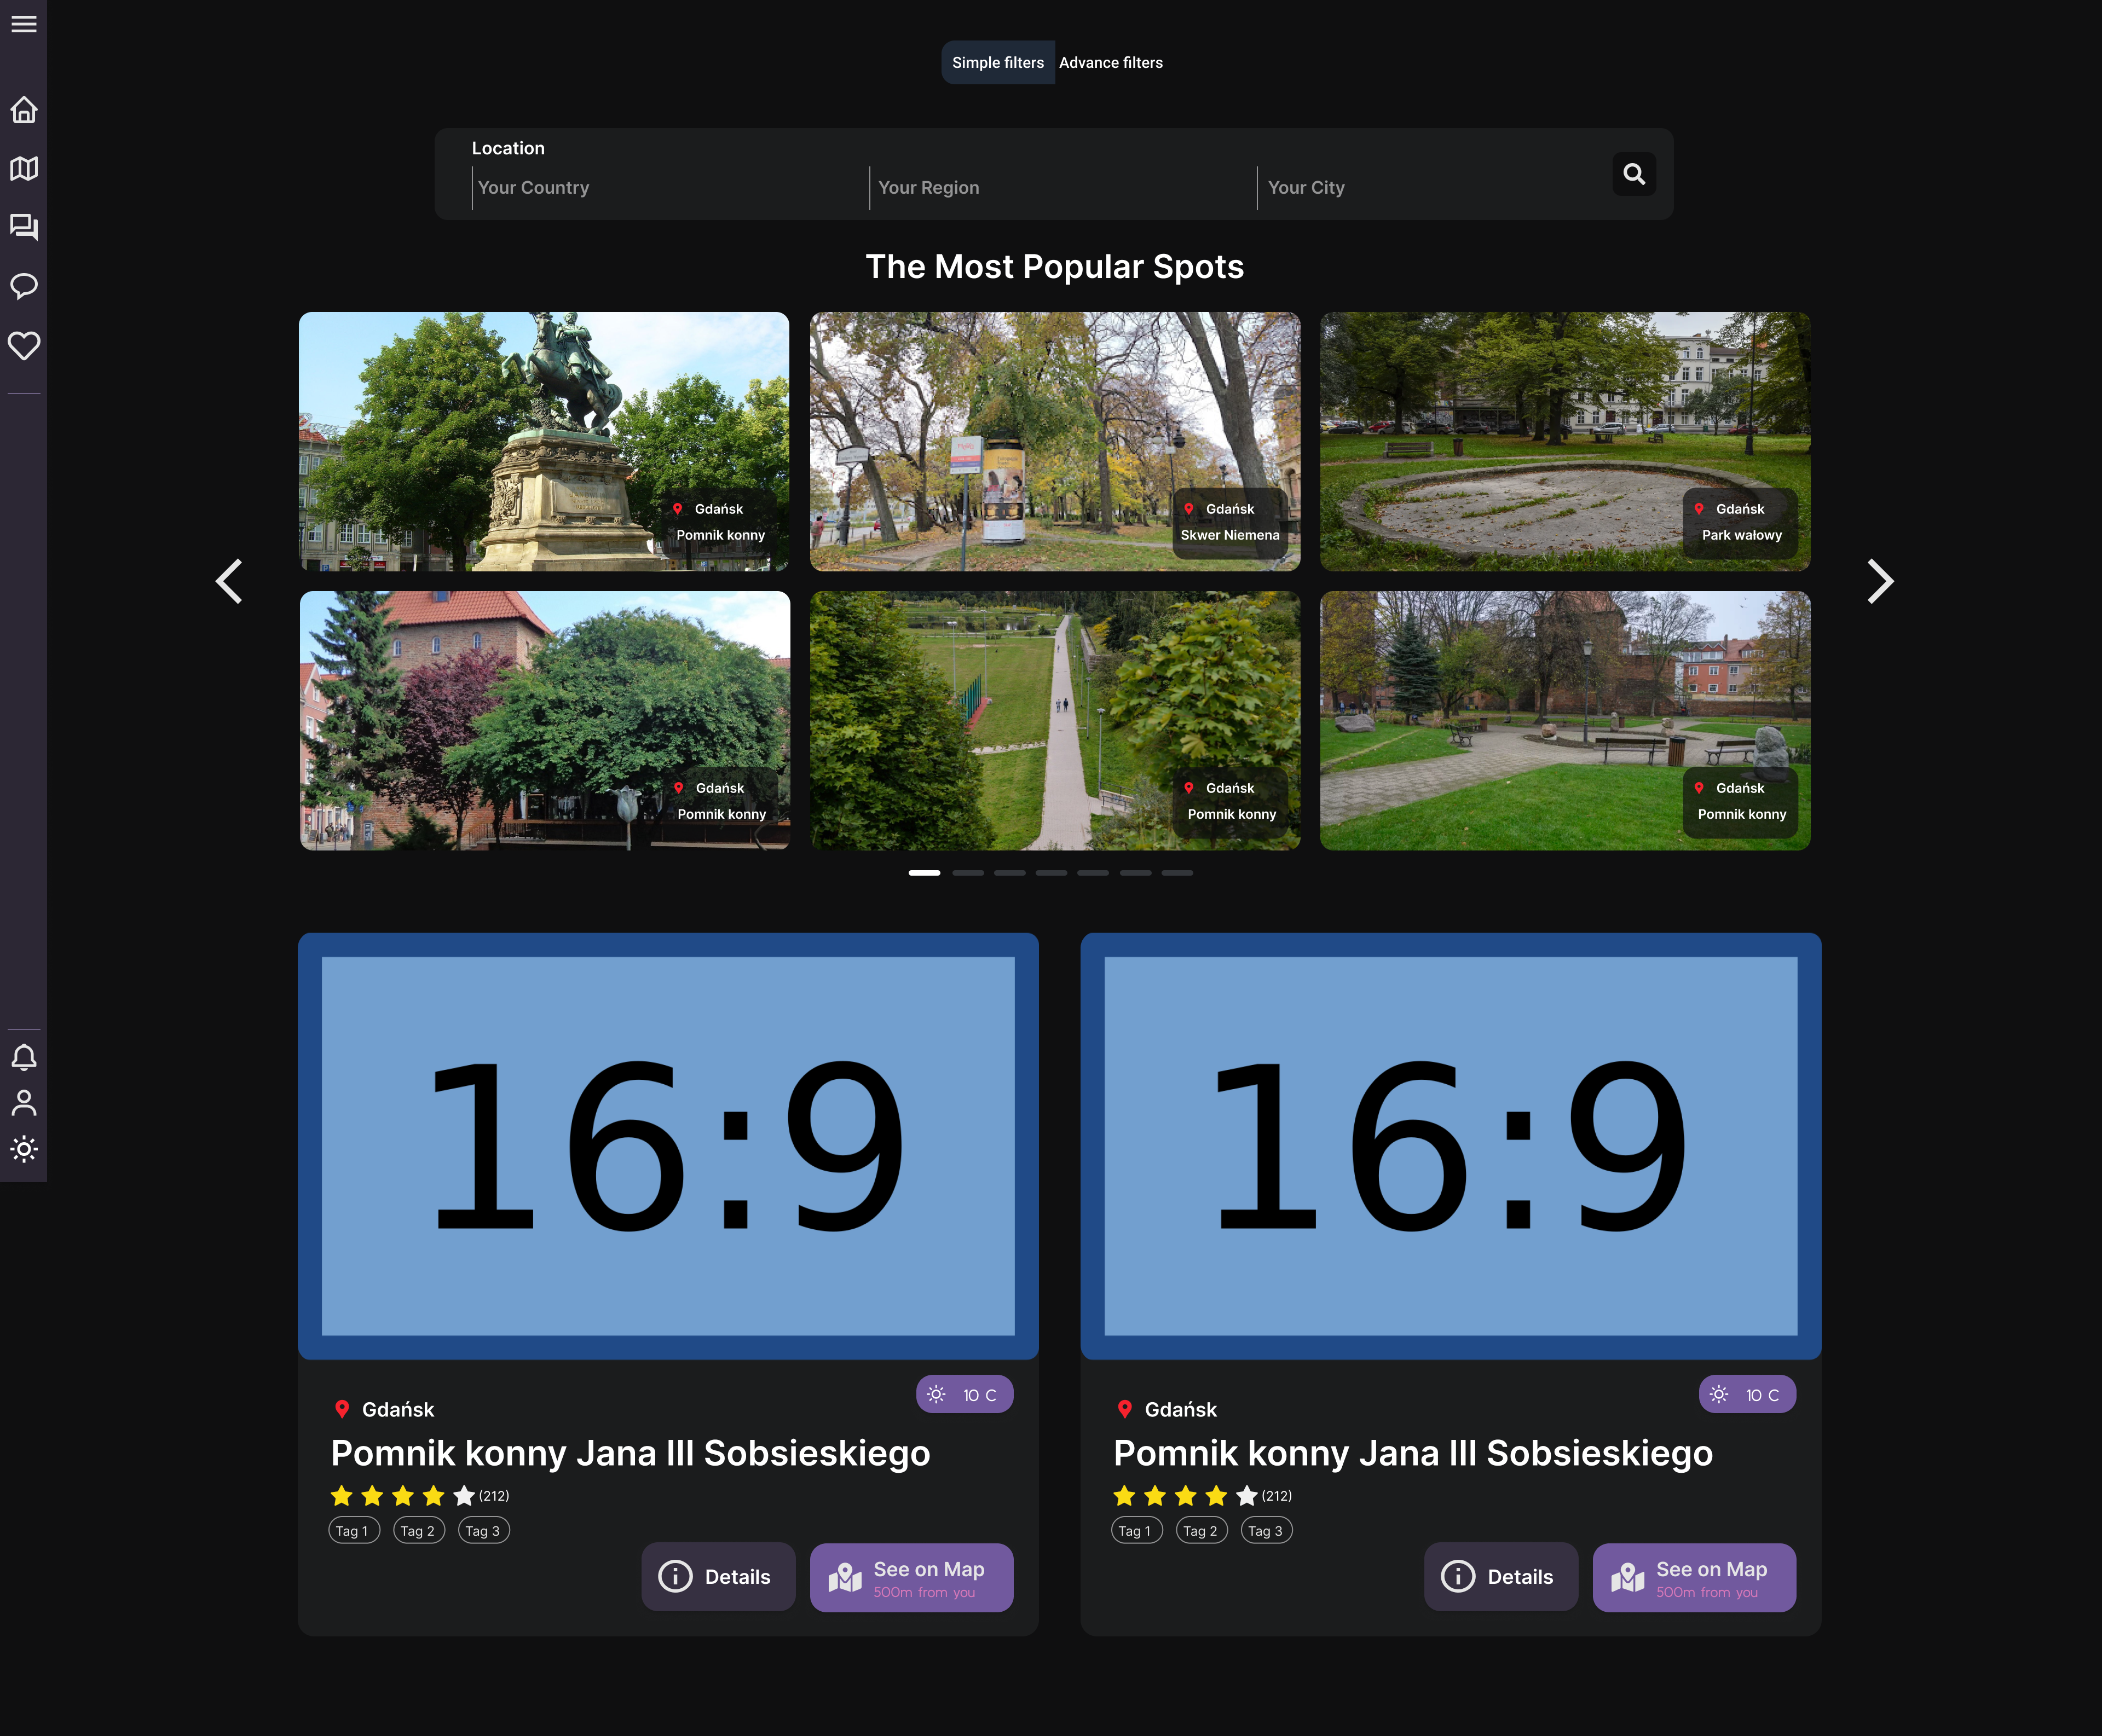
\includegraphics[width=1\textwidth]{attachments/projekt/architektura-interfejsu-uzytkownika/simple-home-page}
    \caption{Projekt prostej strony głównej}
    \label{img:simple-home-page}
\end{figure}

\begin{figure}[H]
    \centering
    \includegraphics[width=1\textwidth]{attachments/projekt/architektura-interfejsu-uzytkownika/advance-home-page}
    \caption{Projekt zaawansowanej strony głównej (1)}
    \label{img:advance-home-page}
\end{figure}

W obu widokach, w górnej części strony, umieszczono przyciski służące do
przełączania się między trybem prostym a zaawansowanym.
Poniżej znajduje się wyszukiwarka \glslink{spot}{spotów}, której układ zależy od wybranego trybu.
Dla prostego widoku przewidziano trzy pola tekstowe do podania kolejno:
kraju, regionu oraz miasta; każde z nich zawiera również listę z
podpowiedziami odpowiadających im lokalizacji.
Dla widoku zaawansowanego zaprojektowano pojedyncze pole do wpisania miasta
oraz listę umożliwiającą wybór dostępnych tagów.
Dodatkowo udostępniono możliwość sortowania wyników według oceny oraz
filtrowania ich z uwzględnieniem minimalnej i maksymalnej oceny (rys. \ref{img:advance-home-page-dropdowns}).

\begin{figure}[H]
    \centering
    \includegraphics[width=1\textwidth]{attachments/projekt/architektura-interfejsu-uzytkownika/advance-home-page-dropdowns}
    \caption{Projekt zaawansowanej strony głównej (2)}
    \label{img:advance-home-page-dropdowns}
\end{figure}

W trybie prostym przewidziano karuzelę z najpopularniejszymi \glslink{spot}{spotami},
dzięki czemu możliwe jest szybkie odnalezienie interesujących miejsc bez
konieczności przeglądania całej listy wyników.

Na dole strony umieszczono listę wyszukanych \glslink{spot}{spotów}.
Każdy kafelek reprezentujący \glslink{spot}{spot} zawiera następujące informacje:
\begin{itemize}
    \item nazwę miasta, w którym znajduje się \glslink{spot}{spot},
    \item nazwę \glslink{spot}{spota},
    \item informacje pogodowe (typ pogody oraz aktualna temperatura),
    \item średnią ocenę oraz liczbę wystawionych opinii,
    \item listę tagów opisujących \glslink{spot}{spota},
    \item przycisk przejścia do widoku szczegółów,
    \item przycisk wyświetlenia \glslink{spot}{spota} na mapie wraz z informacją o
    przybliżonej odległości od bieżącej lokalizacji użytkownika.
\end{itemize}

Oba warianty strony utrzymano w ciemnej kolorystyce, spójnej z pozostałymi
elementami \gls{ui} aplikacji.
Układ komponentów zaplanowano tak, aby zachować czytelność i hierarchię
informacji, a także umożliwić wygodne
korzystanie z aplikacji na ekranach o różnej rozdzielczości.
